% ============================================================================
%  EVNet Sentinel — IEEE Conference Research Paper, v2
%
%  A Leakage-Corrected Reproduction Study of Online Intrusion Detection
%  on Electric Vehicle Charging Networks using CICEVSE2024
%
%  v2 (1 Oct 2026) over v1 (29 Sep): shorter related-work section; adds the
%  testbed attack routes, per-attack testing, error structure, feature
%  separability, naming-confidence trade-off and response guidance; corrects
%  the deployment model (passive mirror-port IDS) and the frontend description.
%  Figures are generated by src/evaluation/make_paper_figures.py.
%
%  Template: IEEE Conference (IEEEtran)    Page limit: 8
%  Build:    pdflatex EVNet_Sentinel_Research_Paper_v2.tex  (run twice)
% ============================================================================
\documentclass[conference]{IEEEtran}
\IEEEoverridecommandlockouts

\usepackage{cite}
\usepackage{amsmath,amssymb,amsfonts}
\usepackage{graphicx}
\graphicspath{{../figures/}}
\usepackage{textcomp}
\usepackage{xcolor}
\usepackage{booktabs}
\usepackage{hyperref}
\usepackage{microtype}
\usepackage{tabularx}

\hypersetup{
    colorlinks=true, linkcolor=blue, urlcolor=blue, citecolor=blue,
    pdftitle={EVNet Sentinel: Leakage-Corrected Intrusion Detection for EV Charging Networks},
    pdfauthor={Varak, Chaurasiya, Chogale, Chavhan}
}

\newcommand{\col}[1]{\texttt{\small #1}}
% Left-aligned flexible column: justified text in narrow table cells spreads badly.
\newcolumntype{L}{>{\raggedright\arraybackslash}X}

\begin{document}

\title{EVNet Sentinel: A Leakage-Corrected Reproduction and Comparative Study of Intrusion Detection on Electric Vehicle Charging Networks}

\author{
\IEEEauthorblockN{Mukta Varak}
\IEEEauthorblockA{\textit{Dept.\ of Computer Engineering} \\
\textit{Vidyalankar Institute of Technology}\\
Mumbai, India \\
24102A0013}
\and
\IEEEauthorblockN{Shruti Chaurasiya}
\IEEEauthorblockA{\textit{Dept.\ of Computer Engineering} \\
\textit{Vidyalankar Institute of Technology}\\
Mumbai, India \\
24102A0018}
\and
\IEEEauthorblockN{Shardul Chogale}
\IEEEauthorblockA{\textit{Dept.\ of Computer Engineering} \\
\textit{Vidyalankar Institute of Technology}\\
Mumbai, India \\
24102A0021}
\and
\IEEEauthorblockN{Neha Chavhan}
\IEEEauthorblockA{\textit{Dept.\ of Computer Engineering} \\
\textit{Vidyalankar Institute of Technology}\\
Mumbai, India \\
24102A0022}
}

\maketitle

% ============================================================================
\begin{abstract}
Electric Vehicle Charging Stations (EVCS) are networked computers whose compromise can halt charging and billing. We present EVNet Sentinel, a network Intrusion Detection System (IDS) for the link between charging stations (EVSE) and their Charging Station Management System (CSMS), and use it to reproduce and audit the online-learning IDS of Makhmudov et al.\ (2025) on CICEVSE2024. We find that the published preprocessing retains capture-session timestamps: a decision tree given the single column \col{bidirectional\_first\_seen\_ms} recovers the 15-class label at 0.9976 accuracy, above the published 0.9840. With the leak removed and results averaged over three seeds, volumetric floods remain perfectly separable ($F_1 = 1.000$) while the six nmap reconnaissance modes are not ($F_1 = 0.183$). We show that this ceiling is a property of the features: within denial-of-service flows the best single feature resolves 98\% of the label uncertainty, within reconnaissance only 5\%. A per-attack test harness finds that no model lets an attack through as normal traffic ($\geq 99.9\%$ flagged), that scans are recognised as reconnaissance 96\% of the time but named only 34\%, and that Random Forest combines the best naming with the fewest false alarms (2\% against 59\% for SVM). We also show that the drift detector fires on capture-file seams rather than on traffic evolution, and we derive from the raw captures that every attack in the dataset targets a charging station. The system is delivered with a prediction API, response guidance per role, and an interactive web front end built on real held-out flows.
\end{abstract}

\begin{IEEEkeywords}
Intrusion detection, EV charging infrastructure, CICEVSE2024, data leakage, adaptive random forest, ADWIN, OCPP
\end{IEEEkeywords}

% ============================================================================
\section{Introduction}

Public EV charging relies on two protocols: ISO~15118 between vehicle and station, and the Open Charge Point Protocol (OCPP) between station and CSMS, which carries authorisation, metering and remote control. Both expose charging networks to denial of service and reconnaissance \cite{b1,b3}. Makhmudov et al.\ \cite{b4} proposed the first online-learning IDS for this setting, an Adaptive Random Forest (ARF) with ADWIN drift detection, reporting 99.13\% binary and 98.40\% multiclass accuracy on CICEVSE2024.

We reproduce that work and find the reported accuracy largely an artefact of the dataset's assembly. Our contributions are:
\begin{enumerate}
    \item \textbf{Leakage audit.} Four verifiable findings: timestamp leakage, a discarded legitimate feature, label autocorrelation in stream order, and drift alarms on capture seams (Section~\ref{sec:leakage}).
    \item \textbf{Corrected, multi-seed benchmarks} of four static classifiers and ARF+ADWIN (Section~\ref{sec:results}).
    \item \textbf{An explanation of the reconnaissance ceiling} from confusion structure and per-feature separability (Section~\ref{sec:why}).
    \item \textbf{Per-attack evaluation}: which model to trust for which attack, false-alarm rates, and how confident a model must be before naming an attack (Section~\ref{sec:perattack}).
    \item \textbf{A working system}: a passive IDS with a prediction API, role-based response guidance and an interactive front end (Section~\ref{sec:system}).
\end{enumerate}

% ============================================================================
\section{Related Work}

Bean et al.\ \cite{b1} survey ML-based IDS for EV charging, identify CICEVSE2024 as the dominant benchmark and ensemble methods as the strongest on flow data, and list concept drift as an open challenge; they do not audit the reported accuracies. Joglekar et al.\ \cite{b2} combine a network and a host IDS; their XGBoost network component reaches 99.99\% after removing IP and MAC identifiers, but timestamps are retained and training is offline. Makhmudov et al.\ \cite{b4}, our baseline, introduce ARF with ADWIN for streaming detection. Malimage et al.\ \cite{b3} motivate the problem from real incidents and regulation without proposing a detector, and Tanyildiz et al.\ \cite{b5} predict the time to the next attack with GAN-augmented deep models on a different dataset. Table~\ref{tab:related} summarises the gap: no prior work audits the CICEVSE2024 preprocessing for leakage, reports variance across seeds, or evaluates per attack.

\begin{table}[htbp]
\caption{Related work on EVCS intrusion detection}
\label{tab:related}
\centering
\footnotesize
\begin{tabularx}{\columnwidth}{@{}lLrcc@{}}
\toprule
\textbf{Work} & \textbf{Approach} & \textbf{Reported} & \textbf{Online} & \textbf{Leak audit} \\
\midrule
Bean \cite{b1}      & Survey (24 studies)        & ---          & ---        & $\times$ \\
Joglekar \cite{b2}  & NIDS+HIDS, XGBoost         & 99.99\%      & $\times$   & IP/MAC only \\
Makhmudov \cite{b4} & ARF + ADWIN                & 98.40\%      & \checkmark & $\times$ \\
Tanyildiz \cite{b5} & GAN + DL, time-to-attack   & $R^2$ 0.74   & $\times$   & --- \\
\midrule
\textbf{This work}  & \textbf{Audit; 4 models + ARF} & \textbf{0.558 m-$F_1$} & \checkmark & \checkmark \\
\bottomrule
\end{tabularx}
\end{table}

% ============================================================================
\section{Dataset and Testbed}
\label{sec:dataset}

\subsection{CICEVSE2024}

The network-traffic subset of CICEVSE2024 \cite{b8} holds 59 packet captures recorded against two charging stations, EVSE-A and EVSE-B, while idle or charging. Flows were extracted with NFStream (86 features) and are labelled from the capture file name. The 15 classes are five volumetric floods (SYN, TCP, UDP, PSH-ACK, SynonymousIP), six nmap reconnaissance modes (TCP port scan, SYN stealth scan, OS fingerprinting, service-version detection, vulnerability scan, aggressive scan), three low-rate or sparse denial-of-service classes (ICMP flood, ICMP fragmentation, Slowloris) and benign traffic.

\subsection{Who attacks what}
\label{sec:routes}

The dataset documents its devices but not which attacked which. Every flow carries source and destination MAC addresses, so we derived each capture's route (Table~\ref{tab:routes}). \emph{Every attack targets a charging station}; none targets the CSMS or the vehicle. In six captures the vehicle itself is the attacker, scanning EVSE-B over the ISO~15118 link. Traffic was recorded from a mirrored switch port, so a detector trained on it is a \emph{passive} IDS: it observes a copy of the traffic and raises alerts; it cannot block.

\begin{table}[htbp]
\caption{Attack routes, from the MAC addresses in the 57 attack captures}
\label{tab:routes}
\centering
\footnotesize
\begin{tabularx}{\columnwidth}{@{}llrL@{}}
\toprule
\textbf{Attacker} & \textbf{Target} & \textbf{Caps.} & \textbf{Attacks} \\
\midrule
Kali PC (wifi)        & EVSE-A & 24 & all but UDP flood \\
Kali PC (wifi)        & EVSE-B & 23 & all but UDP flood, Slowloris \\
Raspberry Pi (wifi)   & both   & 4  & UDP flood \\
Compromised EV (V2G)  & EVSE-B & 6  & the six scans \\
\bottomrule
\end{tabularx}
\end{table}

\subsection{Corrected preprocessing}

Our pipeline concatenates the captures, drops identifiers, addresses and sparse application-layer fields, then removes the six absolute timestamp columns (\col{*\_first\_seen\_ms}, \col{*\_last\_seen\_ms}) and \col{src\_port}, keeps \col{dst\_port}, and removes constant columns. Global deduplication reduces 2,744,700 flows to \textbf{1,198,151}, with 60 features, standardised and split 70/15/15 with stratification (838,705 / 179,723 / 179,723).

% ============================================================================
\section{Leakage Analysis}
\label{sec:leakage}

\subsection{Finding 1: the label is in one timestamp}

Each attack was captured in its own file at its own time, so absolute timestamps identify the recording, not the traffic. The reference preprocessing \cite{b4} keeps all six. Table~\ref{tab:leak} shows what a depth-25 decision tree recovers from a single feature (15 classes, 3-fold cross-validation): the timestamp alone beats the published model. In our pre-correction Random Forest, 39.8\% of feature importance sat on those six columns.

\begin{table}[htbp]
\caption{Single-feature label recovery}
\label{tab:leak}
\centering
\footnotesize
\begin{tabular}{@{}llr@{}}
\toprule
\textbf{Feature} & \textbf{Nature} & \textbf{Accuracy} \\
\midrule
\col{bidirectional\_first\_seen\_ms} & fingerprint & \textbf{0.9976} \\
\col{src\_port} & partial & 0.4028 \\
\col{dst\_port} & legitimate & 0.2917 \\
\midrule
\multicolumn{2}{@{}l}{\emph{Published multiclass accuracy \cite{b4}}} & \emph{0.9840} \\
\bottomrule
\end{tabular}
\end{table}

\subsection{Finding 2: the legitimate feature is the one discarded}

A $2\times2$ ablation over timestamps and \col{dst\_port} (Table~\ref{tab:ablation}) shows that the published configuration discards \col{dst\_port} --- the feature that defines a port scan --- and keeps the timestamps, so its 273,932 reconnaissance flows are separable by \emph{when} they were captured rather than by what they did.

\begin{table}[htbp]
\caption{Fingerprint ablation: flows remaining after deduplication}
\label{tab:ablation}
\centering
\footnotesize
\begin{tabular}{@{}llrr@{}}
\toprule
\textbf{Timestamps} & \textbf{\col{dst\_port}} & \textbf{Total} & \textbf{Recon.} \\
\midrule
kept & kept & 2,728,799 & 1,724,504 \\
\textbf{kept} & \textbf{dropped} & \textbf{1,277,520} & \textbf{273,932} \\
dropped & kept & 1,198,143 & 194,737 \\
dropped & dropped & 977,862 & 6,821 \\
\bottomrule
\end{tabular}
\end{table}

\subsection{Finding 3: stream order and drift}

In capture order consecutive flows share a label, so a prequential learner scores well by predicting ``what came recently''. On the full 1,921,182-flow leak-free stream, ARF+ADWIN reaches 0.9997 accuracy in capture order but 0.5585 shuffled: a 44-point inflation from autocorrelation alone. In capture order 42 of 43 ADWIN alarms fall within 100 flows of a capture-file boundary, against $2.2 \pm 1.5$ expected at random ($p < 0.0005$; Fig.~\ref{fig:drift}). The detector finds the seams of dataset assembly, not concept drift in charging traffic.

\begin{figure}[htbp]
\centering
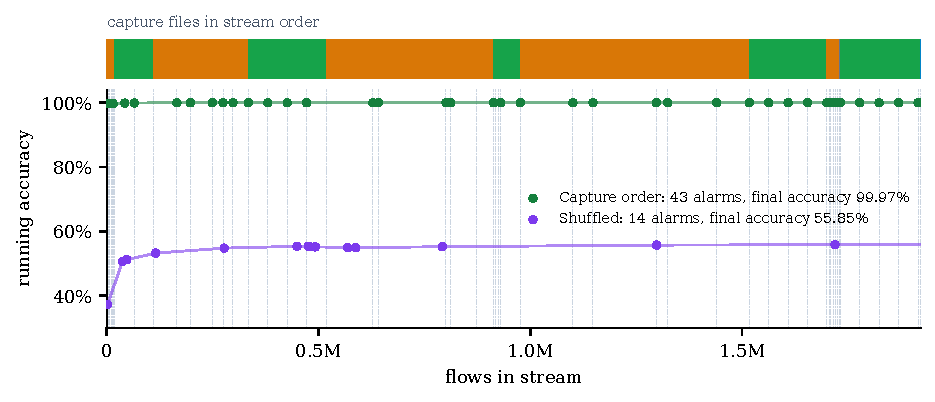
\includegraphics[width=\columnwidth]{fig_drift.pdf}
\caption{ADWIN alarms over the training stream. Top band: the 58 capture files in stream order (green volumetric, orange reconnaissance, grey low-rate, blue benign); dashed lines mark file seams.}
\label{fig:drift}
\end{figure}

\subsection{Finding 4: \col{src\_port} is a residual fingerprint}

Ephemeral source ports are allocated near-sequentially, so they band within a capture. Removing \col{src\_port} with rows and split held fixed lowers macro-$F_1$ by 0.076 for Random Forest but 0.170 for a deeper Decision Tree, after which the two converge (0.5138 and 0.5135): the tree's earlier advantage was memorisation.

% ============================================================================
\section{System}
\label{sec:system}

Fig.~\ref{fig:pipeline} summarises the method. EVNet Sentinel is placed where the dataset was recorded: on the mirrored port of the switch that carries station, CSMS and vehicle traffic, so it sees every flow without being in its path.

\begin{figure*}[htbp]
\centering
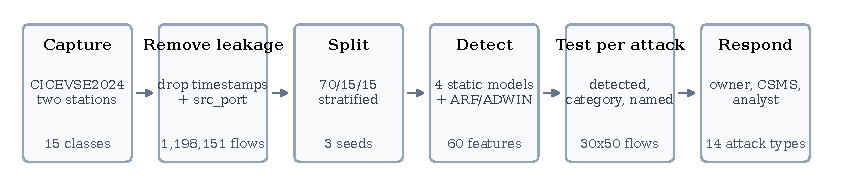
\includegraphics[width=\textwidth]{fig_pipeline.pdf}
\caption{Method at a glance, from capture to response.}
\label{fig:pipeline}
\end{figure*}

\textbf{Models and API.} Static scikit-learn models and the River ARF are trained offline on the corrected features. A FastAPI service loads the models and the matching scaler at start-up and classifies one flow per request; a single command starts it on the corrected models.

\textbf{Response guidance.} Each detection maps to actions for three roles --- the station owner, the CSMS operator and the network analyst --- with severity per attack. When the active model cannot reliably name an attack (per Section~\ref{sec:perattack}), the guidance falls back to the category, because acting on a confidently wrong name is worse than acting on a correct category.

\textbf{Front end.} A Next.js application built entirely from exported results (no live inference) provides: an interactive landing page where visitors aim attacks at a station and see the model's verdict on a real held-out flow, and tune the naming-confidence bar of Section~\ref{sec:confidence}; a simulation console that replays held-out flows from the device that really sent them to the station they really hit (Table~\ref{tab:routes}), with scripted multi-attack campaigns and an incident log; and a dashboard with the findings, per-attack results and figures of this paper.

% ============================================================================
\section{Experimental Methodology}

\textbf{Models.} Random Forest (100 trees, depth 15), Decision Tree (depth 20), Logistic Regression and a linear SVM (SGD with log and hinge loss), all class-balanced; and ARF \cite{b6} implemented in River \cite{b9} (20 trees, \col{max\_features}=0.5, grace period 30, ADWIN \cite{b7} with $\delta = 0.002$), the configuration of \cite{b4}.

\textbf{Protocol.} Every headline number is the mean $\pm$ standard deviation over seeds 42, 1337 and 2024, each varying both the split and the model initialisation; with classes of 28--81 flows, a single seed is unreliable. Macro-$F_1$ is the headline metric because accuracy is dominated by floods: the corrected Random Forest scores 0.868 accuracy but 0.558 macro-$F_1$ on the same predictions.

\textbf{Per-attack testing.} Each attack type is fed to every model in 30 random batches of 50 unseen flows, for each of the three trained model sets. Each verdict is scored at three levels: \emph{detected} (flagged as malicious at all), \emph{category} (denial of service vs.\ reconnaissance) and \emph{exact} (named correctly). Benign traffic is scored on false alarms. Mixed campaigns send four attacks at once (25 flows each, 30 trials). The harness fails if a regression gate is crossed: each flood named exactly at $\geq 0.95$, each attack detected at $\geq 0.95$ and each scan categorised at $\geq 0.85$ by at least one model.

% ============================================================================
\section{Results and Discussion}
\label{sec:results}

\subsection{Corrected benchmarks}

\begin{table}[htbp]
\caption{Multiclass results (mean $\pm$ std over 3 seeds)}
\label{tab:results}
\centering
\footnotesize
\begin{tabular}{@{}lrrrr@{}}
\toprule
\textbf{Model} & \textbf{Macro-$F_1$} & \textbf{W-$F_1$} & \textbf{Acc.} & \textbf{Fit (s)} \\
\midrule
Random Forest & \textbf{0.558$\pm$0.008} & 0.865 & 0.868 & 8.5 \\
Decision Tree & 0.557$\pm$0.010 & 0.868 & 0.868 & 3.4 \\
Log.\ Regression & 0.436$\pm$0.017 & 0.853 & 0.863 & 78.9 \\
SVM & 0.411$\pm$0.017 & 0.849 & 0.862 & 34.9 \\
\bottomrule
\end{tabular}
\end{table}

Random Forest and Decision Tree are indistinguishable within one standard deviation (Table~\ref{tab:results}), confirming Finding~4. Removing the timestamps cost Random Forest 0.365 macro-$F_1$ on a like-for-like split, whereas the linear models barely moved (Table~\ref{tab:leakeffect}): a hyperplane cannot exploit a timestamp axis the way a tree can.

\begin{table}[htbp]
\caption{Macro-$F_1$ before and after removing the timestamps}
\label{tab:leakeffect}
\centering
\footnotesize
\begin{tabular}{@{}lrrr@{}}
\toprule
\textbf{Model} & \textbf{Leaked} & \textbf{Corrected} & \textbf{$\Delta$} \\
\midrule
Random Forest & 0.9547 & 0.5894 & $\mathbf{-0.3653}$ \\
Log.\ Regression & 0.4622 & 0.3308 & $-0.1314$ \\
SVM & 0.2829 & 0.3084 & $+0.0255$ \\
\bottomrule
\end{tabular}
\end{table}

\subsection{Per-class results: the reconnaissance ceiling}

\begin{table}[htbp]
\caption{Per-class $F_1$, Random Forest, mean over 3 seeds}
\label{tab:perclass}
\centering
\footnotesize
\begin{tabular}{@{}llrr@{}}
\toprule
\textbf{Class} & \textbf{Group} & \textbf{Support} & \textbf{$F_1$} \\
\midrule
PSH-ACK flood & DoS & 195,952 & 1.000 \\
SynonymousIP flood & DoS & 256,739 & 1.000 \\
TCP flood & DoS & 256,297 & 1.000 \\
SYN flood & DoS & 259,484 & 1.000 \\
UDP flood & DoS & 32,072 & 0.999 \\
\midrule
TCP port scan & Recon. & 35,123 & 0.265 \\
OS fingerprinting & Recon. & 27,702 & 0.223 \\
Vulnerability scan & Recon. & 39,002 & 0.204 \\
Service-version detection & Recon. & 30,338 & 0.156 \\
Aggressive scan & Recon. & 27,815 & 0.145 \\
SYN stealth scan & Recon. & 34,765 & 0.105 \\
\midrule
Benign & Other & 81 & 0.986 \\
ICMP flood & Other & 32 & 0.660 \\
ICMP fragmentation & Other & 28 & 0.439 \\
Slowloris & Other & 2,721 & 0.191 \\
\bottomrule
\end{tabular}
\end{table}

Volumetric floods reach $F_1 = 1.000$ with zero variance across seeds; reconnaissance averages 0.183 (Table~\ref{tab:perclass}). Support does not explain the gap: UDP flood (32,072 flows) scores 0.999 while TCP port scan (35,123) scores 0.265.

\subsection{Why the scans cannot be separated}
\label{sec:why}

\begin{figure}[htbp]
\centering
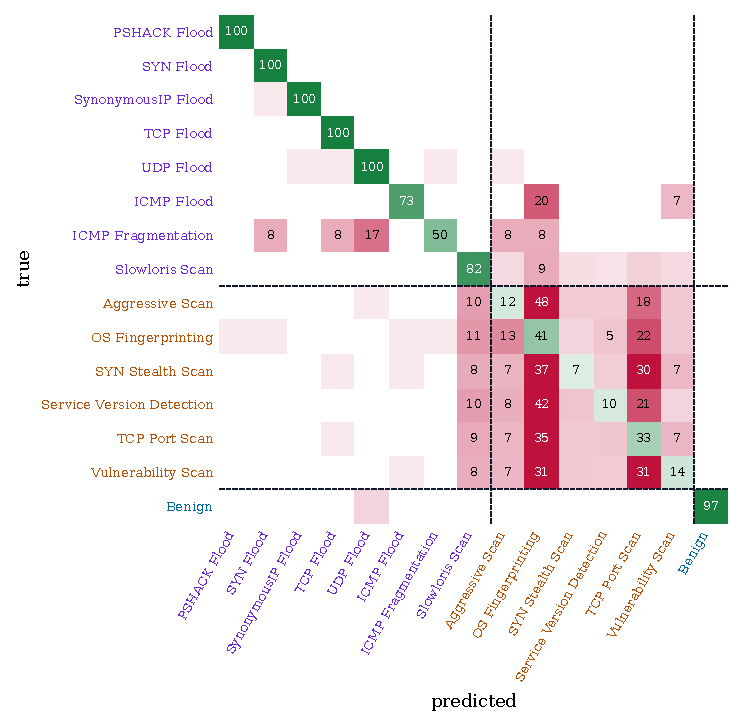
\includegraphics[width=\columnwidth]{fig_confusion_rf.pdf}
\caption{Random Forest confusion matrix, row-normalised and averaged over three seeds (\%; cells under 5\% unlabelled). Dashed lines separate denial of service, reconnaissance and benign.}
\label{fig:confusion}
\end{figure}

The errors have structure (Fig.~\ref{fig:confusion}). Scans collapse into one scan: Random Forest calls 32--48\% of every other scan \emph{OS fingerprinting}, while Logistic Regression absorbs them into \emph{TCP port scan}; which class becomes the sink depends on the model, but a sink exists for all of them. One confusion crosses the category line: 8--11\% of every scan is called Slowloris by Random Forest (3\% by Logistic Regression), as both hold long-lived, near-idle connections.

To test whether this is a limit of the models or of the data, we measure, within each category, the share of label uncertainty that each feature removes on its own, $I(X_j;Y)/H(Y)$ (Fig.~\ref{fig:separability}). Inside denial of service one inter-arrival-time feature resolves 98\%; inside reconnaissance the best feature resolves 5\%. No flow statistic separates the six nmap modes --- \texttt{nmap -A} is itself a superset of two other modes --- so no model trained on these features can. Permutation importance, tried first, reads near zero for every scan feature because the features are redundant; mutual information answers the question directly.

\begin{figure*}[htbp]
\centering
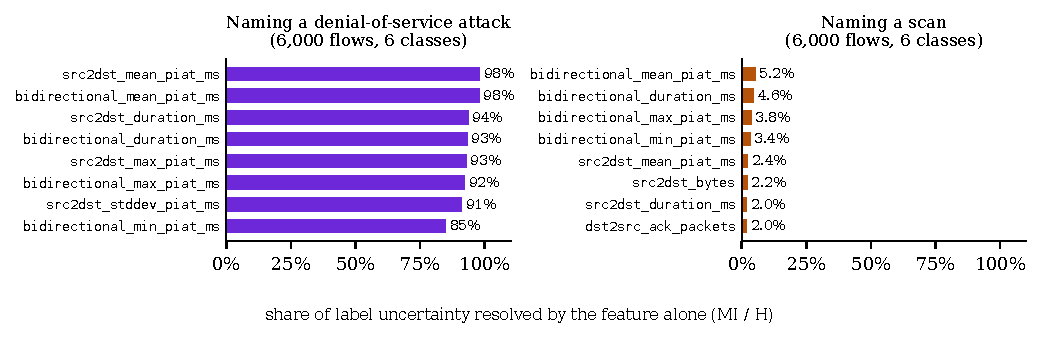
\includegraphics[width=0.86\textwidth]{fig_separability.pdf}
\caption{Per-feature separability inside denial-of-service and inside reconnaissance flows (6,000 held-out flows each). Both panels share one axis.}
\label{fig:separability}
\end{figure*}

\subsection{Per-attack detection and model choice}
\label{sec:perattack}

\begin{table}[htbp]
\caption{Per-attack test: exact-name rate for Random Forest, and the best model at naming (exact) and at categorising (cat.)}
\label{tab:perattack}
\centering
\footnotesize
\begin{tabular}{@{}lrlrl@{}}
\toprule
\textbf{Attack} & \textbf{RF} & \textbf{Best exact} & & \textbf{Best cat.} \\
\midrule
5 volumetric floods & 1.00 & all tie & 1.00 & all \\
Slowloris & 0.82 & RF & 0.82 & RF \\
ICMP flood$^*$ & 0.74 & RF & 0.74 & RF \\
ICMP fragmentation$^*$ & 0.49 & LR 0.58 & 0.82 & SVM \\
\midrule
TCP port scan & 0.32 & LR 0.65 & 0.97 & LR \\
SYN stealth scan & 0.06 & SVM 0.43 & 0.97 & LR \\
OS fingerprinting & 0.41 & RF/DT 0.41 & 0.95 & LR \\
Vulnerability scan & 0.13 & SVM 0.26 & 0.97 & LR \\
Aggressive scan & 0.12 & DT 0.15 & 0.94 & LR \\
Service-version det. & 0.10 & DT 0.13 & 0.96 & LR \\
\bottomrule
\multicolumn{5}{@{}l}{\scriptsize $^*$Fewer than 100 held-out flows; resampled.}
\end{tabular}
\end{table}

No attack slips through: across 90 mixed campaigns every model flags at least 99.9\% of attack flows as malicious, so the system's weakness is \emph{naming}, not noticing. Every model names the five floods exactly at 0.98 or better. Scans are recognised as reconnaissance 96\% of the time by the best model for each, but named only 34\% (Table~\ref{tab:perattack}), and no single model is best at naming them. False alarms on benign traffic separate the models sharply: 2\% for Random Forest, 12\% for Decision Tree, 46\% for Logistic Regression and 59\% for SVM (36 benign flows in total; indicative). We therefore recommend \textbf{Random Forest as the primary detector} --- it names attacks as well as any model and raises the fewest false alarms --- with Logistic Regression as a second opinion on whether traffic is a scan, where it is best on all six.

\subsection{How sure before naming?}
\label{sec:confidence}

The response guidance acts on the category when a name is unreliable. We quantify the trade-off by naming an attack only when the model's top-class probability exceeds a bar $t$, and reporting the category otherwise. For Random Forest, scans at $t = 0$ are named correctly 19\% of the time and \emph{wrongly} 81\%; at $t = 0.5$ wrong names fall to 3\%, and 94\% are reported as ``reconnaissance'' --- correct and actionable. Denial of service keeps 93\% exact naming at the same bar. A single Decision Tree cannot express doubt this way: some scans stay confidently wrong even at $t = 0.99$. (Logistic Regression is excluded: its multiclass probabilities saturate, so their arg-max disagrees with its own predictions.)

% ============================================================================
\section{Reproducibility}

All results regenerate from the public repository\footnote{\url{https://github.com/Mukta01/EVNet\_Sentinel}} with pinned dependencies (River's API changed materially around 0.21). Key scripts: \col{preprocess.py} (corrected pipeline); \col{run\_experiments.py} (multi-seed results and models); \col{attack\_test\_harness.py} (per-attack tests, regression gates); \col{replay\_reference\_preprocessing.py}, \col{ablate\_fingerprints.py}, \col{srcport\_control.py}, \col{drift\_boundary\_alignment.py} (Findings~1--4); \col{attack\_routes.py} (Table~\ref{tab:routes}); and \col{make\_paper\_figures.py}, which draws every figure from the same exported data the front end displays.

% ============================================================================
\section{Limitations}

\begin{enumerate}
    \item \textbf{Label noise.} Labels come from capture file names, so background traffic recorded during an attack carries the attack label; part of the reconnaissance confusion may be such flows.
    \item \textbf{Benign sparsity.} Only 81 benign flows exist, so binary attack-vs-benign classification is trivial and excluded, and false-alarm rates are indicative.
    \item \textbf{Random split.} Headline results use a stratified random split for comparability; grouped and temporal splits are implemented but not reported here.
    \item \textbf{One testbed.} Two stations, one CSMS and standard attack tools at default settings; a paced or disguised scan changes exactly the timing features the detector relies on.
    \item \textbf{Untested responses and unexplored modalities.} The response guidance is standard practice, not measured here; CICEVSE2024's host-event and power traces, which may separate the scans, are unused.
\end{enumerate}

% ============================================================================
\section{Conclusion}

The high accuracies reported for ML-based intrusion detection on CICEVSE2024 are largely an artefact of capture timestamps: one timestamp column beats the published model. With the leak removed, volumetric floods remain trivially separable while the six nmap scan modes are not, and per-feature separability shows this is a property of flow statistics rather than of model capacity. Operationally, no attack goes unnoticed, Random Forest names attacks as well as any model with the fewest false alarms, and requiring confidence before naming turns most wrong scan names into correct category alerts. The drift detector, on ordered streams, fires on dataset seams. Future work should model packet sequences within a flow, which flow aggregation discards; fuse host and power data; and evaluate on grouped splits and against an autocorrelation baseline.

\section*{Acknowledgment}

We build on the open-source implementation of \cite{b4} and thank the Canadian Institute for Cybersecurity for CICEVSE2024. This work was carried out for the Software Engineering course at Vidyalankar Institute of Technology.

% ============================================================================
\begin{thebibliography}{00}

\bibitem{b1} J.\ Bean, V.\ Manias et al., ``Cybersecurity of electric vehicle charging infrastructure: Recent advances, open challenges, and future directions,'' arXiv:2605.24190v1, May 2026.

\bibitem{b2} C.\ Joglekar et al., ``A hybrid intrusion detection system for electric vehicle charging infrastructure,'' arXiv:2606.23236v1, 2026.

\bibitem{b3} K.\ Malimage et al., ``Cybersecurity challenges in the electric vehicle market,'' in \emph{Proc.\ CIGRE Canada Conference}, 2023, pp.\ 1--6.

\bibitem{b4} F.\ Makhmudov, D.\ Kilichev, U.\ Giyosov, and F.\ Akhmedov, ``Online machine learning for intrusion detection in electric vehicle charging systems,'' \emph{Mathematics}, vol.\ 13, no.\ 5, p.\ 712, 2025, DOI: 10.3390/math13050712.

\bibitem{b5} E.\ Tanyildiz et al., ``Detection of cyber attacks in electric vehicle charging systems using a remaining useful life generative adversarial network,'' \emph{Scientific Reports}, vol.\ 15, 2025.

\bibitem{b6} H.\ M.\ Gomes, A.\ Bifet, J.\ Read, J.\ P.\ Barddal, F.\ Enembreck, B.\ Pfharinger, G.\ Holmes, and T.\ Abdessalem, ``Adaptive random forests for evolving data stream classification,'' \emph{Machine Learning}, vol.\ 106, no.\ 9--10, pp.\ 1469--1495, 2017.

\bibitem{b7} A.\ Bifet and R.\ Gavald\`{a}, ``Learning from time-changing data with adaptive windowing,'' in \emph{Proc.\ SIAM Int.\ Conf.\ Data Mining (SDM)}, 2007, pp.\ 443--448.

\bibitem{b8} Canadian Institute for Cybersecurity, ``CICEVSE2024 dataset,'' University of New Brunswick, 2024. [Online]. Available: \url{https://www.unb.ca/cic/datasets/}

\bibitem{b9} J.\ Montiel, M.\ Halford, S.\ M.\ Mastelini et al., ``River: Machine learning for streaming data in Python,'' \emph{J.\ Mach.\ Learn.\ Res.}, vol.\ 22, no.\ 110, pp.\ 1--8, 2021.

\end{thebibliography}

\end{document}
